Dieser Abschnitt unserer Arbeit befasst sich mit dem entwickelten
GUI. Benutzeroberfl{\"a}che zu Programmieren, durch welche eine Chat
Kommunikation via CRODT Protokoll vorgenommen werden kann. Hierbei galt es
Grundlegende Betrachtungen bez{\"u}glich des Interfaces anzustellen. Auf Basis
der Design Regeln nach Nielsen wurde der erste Prototyp entwickelt. Das GUI
besteht aus dem Empfangsfenster (Abb 1. oben links) dem Eingabenfenster (Abb 1.
unten links) sowie der Priorit{\"a}tenliste (Abb 1. oben rechts) und den
Bedienelementen (Abb 1. unten rechts). Die Implementierung erfolgte dabei in
C++ durch Nutzung der Qt-Bibliothek. Da f{\"u}r unsere Arbeit aufgrund der
begrenzten zeit keine M{\"o}glichkeit f{\"u}r eine Nutzerzentrierte GUI
Entwicklung war, wurde der bereits erw{\"a}hnte Nutzerunabh{\"a}ngige Entwurf
nach Jakob Nielsen gew{\"a}hlt. Dieser Entwurf sieht eine Planung nach zehn
Regeln vor.

Regeln des GUI Designentwurfs nach Jakob Nielsen:

   \begin{enumerate}[I]
     \item Nutzung Einfacher und nat{\"u}rlicher Dialoge
     \item Verwendung der Nutzersprache
     \item Minimierung der Ged{\"a}chtnislast des Nutzers
     \item Nutzung konsistenter Formulierungen
     \item Dem Nutzer stets Feedback geben
     \item Klar markierte Navigationsm{\"o}glichkeiten anbieten
     \item Dem Nutzer Shortcuts anbieten
     \item Lieferung genauer Fehlermeldungen
     \item Vermeidung vermeidbarer Fehler
     \item Bereitstellen einer Hilfe und Dokumentation
   \end{enumerate}

Je nach Komplexit{\"a}t des vorliegenden Projekts gilt es einzelne Punkte
hierbei eventuell schwerer zu gewichten als andere. So steigt z.B. bei
zunehmender Komplexit{\"a}t des GUI die Wichtigkeit einer ausf{\"u}hrlichen
Hilfe und Dokumentation. Da die Komplexit{\"a}t des GUI im Szenario der
Projektarbeit {\"u}berschaubar ist, verzichten wir auf eine Hilfe Funktion und
ersetzen diese durch eine Ausf{\"u}hrliche Dokumentation.

\begin{center}
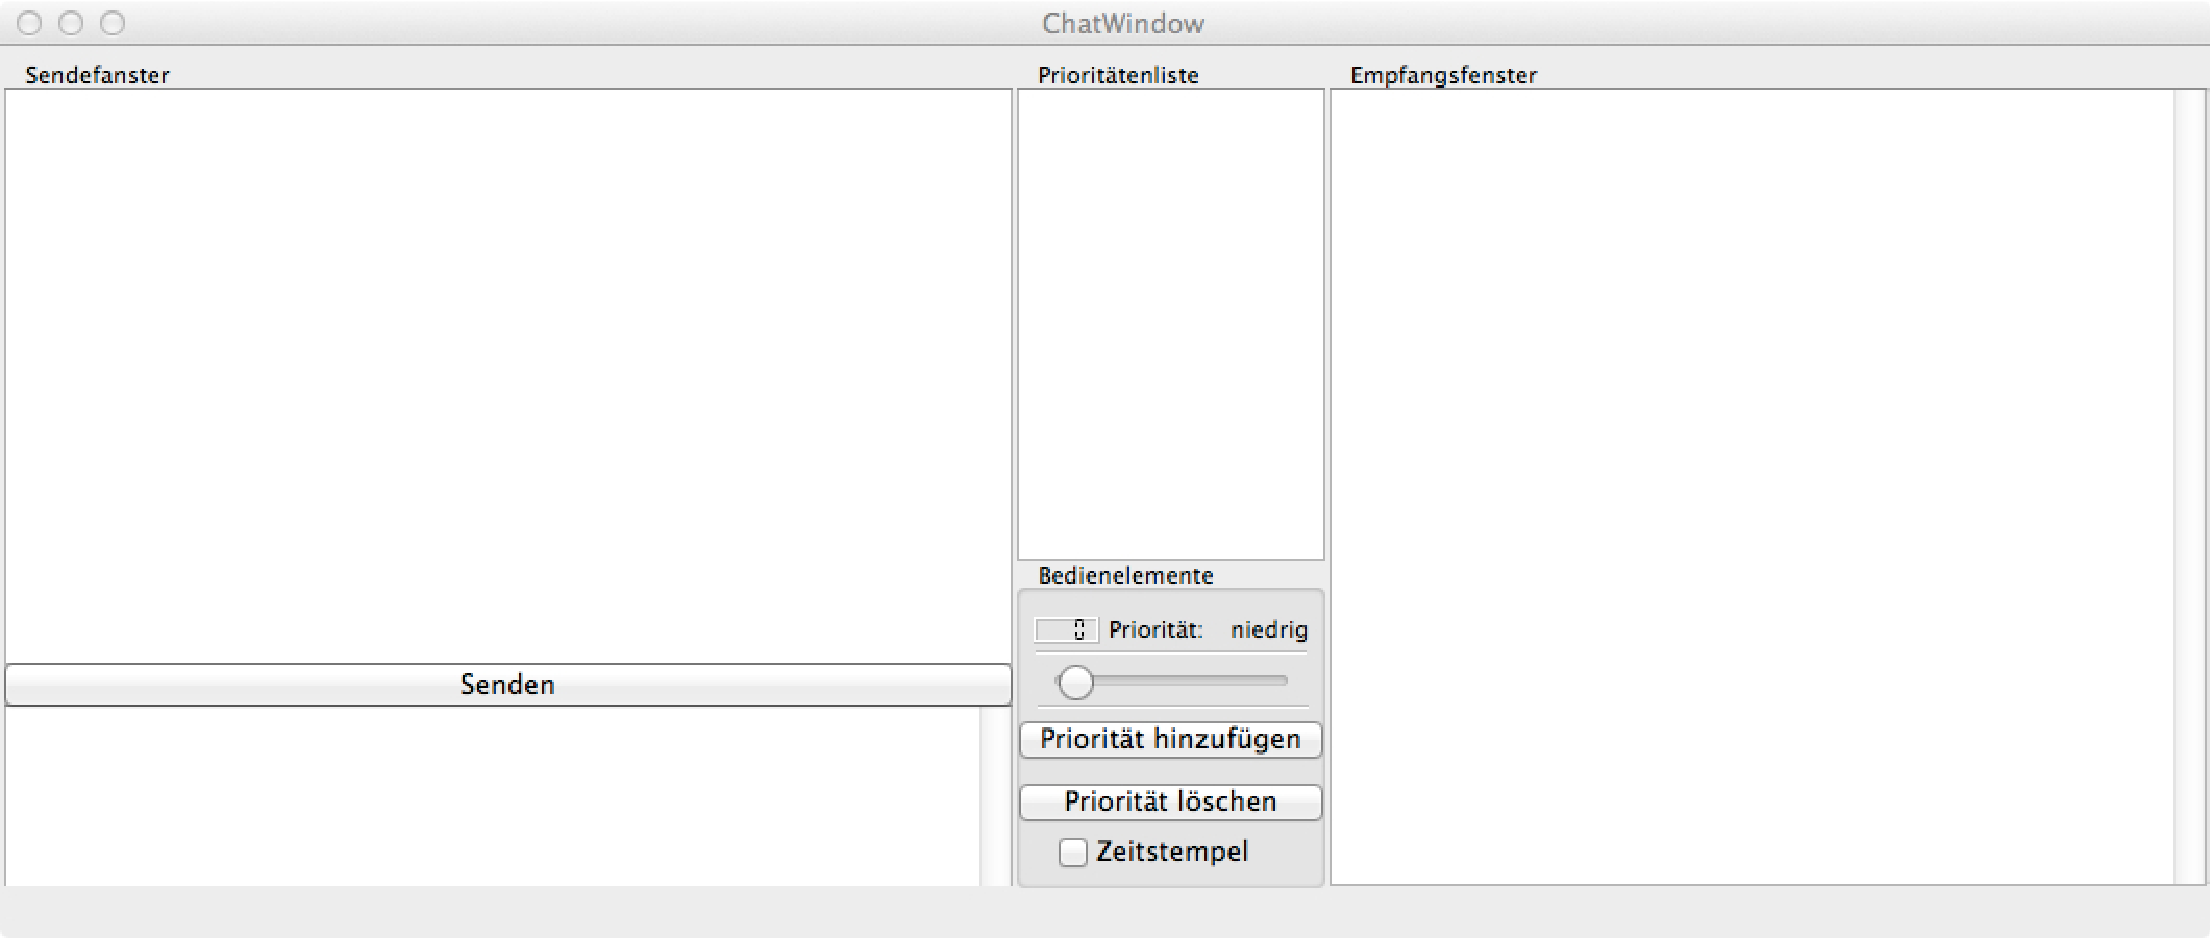
\includegraphics[scale=0.38]{../Bilder/GUI_1.pdf}
\end{center}

\begin{center}
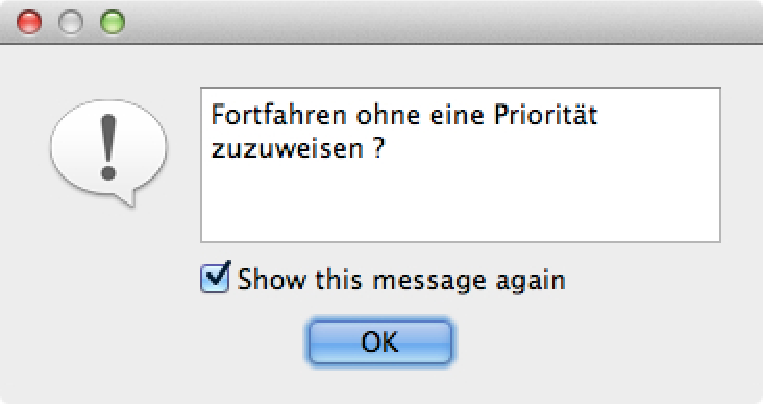
\includegraphics[width=8cm]{../Bilder/Msg_1.pdf}
\end{center}

\begin{center}
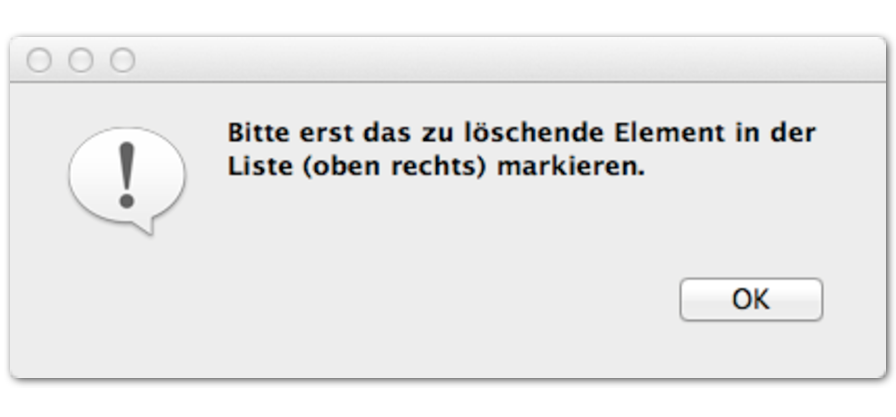
\includegraphics[width=8cm]{../Bilder/Msg_2.pdf}
\end{center}

\begin{center}
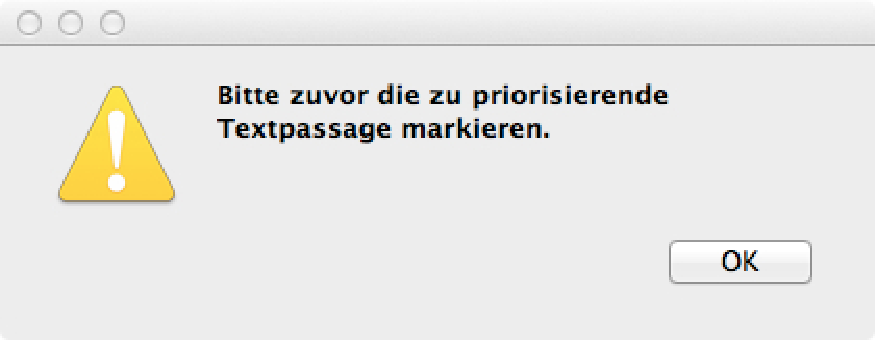
\includegraphics[width=8cm]{../Bilder/Msg_3.pdf}
\end{center}
